\chapter{熱・統計・量子統計力学}
\section{熱力学}
\subsection{状態量}
系の状態のみで一意に決まり, 過去の履歴・経路に依らない(積分値が経路に依らない)ものを状態量と呼ぶ. 
\subsection{完全な熱力学関数}
系の平衡状態における熱力学的性質の情報を全て持っているものを完全な熱力学関数と呼ぶ. 示量性状態量. 系の情報を全て持っているというのは, 状態量がこの関数の偏微分で全て求まるということ. 例えば内部エネルギー$U(S, N, V)$を用いて
\begin{eqnarray}
  \partial_SU &=& T\\
  \partial_NU &=& \mu\\
  \partial_VU &=& -p
\end{eqnarray}
という状態量が求まる. 全微分は
\begin{eqnarray}
  dU = TdS -pdV + \mu dN
\end{eqnarray}
である. これを変形して
\begin{eqnarray}
  dS = \frac{1}{T}dU +\frac{p}{T}dV - \frac{\mu}{T} dN
\end{eqnarray}
となり, $S$は$U, V, N$を変数とする関数として表された時に完全な熱力学関数となる. 統計力学においては温度を定義するときに
\begin{eqnarray}
  \partial_US = \frac{1}{T}
\end{eqnarray}
という表式をしばしば用いる.
\subsection{自由エネルギー}
熱力学第二法則より, 系は自由エネルギーが減少する方向に遷移する. 
\subsubsection{ヘルムホルツ自由エネルギー}
等温下で仕事として取り出し可能なエネルギーを表す.ヘルムホルツエネルギーが極小値を取るとき, 系は熱平衡状態にある.

定義:
\begin{eqnarray}
  F(T, V, N) = U(S(T, V, N), V, N) -TS(T, V, N)
\end{eqnarray}
ここで現れるエントロピーは完全な熱力学関数ではない. 各変数による偏微分は
\begin{eqnarray}
  \partial_TF &=& -S\\
  \partial_VF &=& -p\\
  \partial_NF &=& \mu
\end{eqnarray}
である. 全微分は
\begin{eqnarray}
  dF = -S(T, V, N)dT -p(T, V, N)dV + \mu(T, V, N) dN
\end{eqnarray}
\subsubsection{ギブズ自由エネルギー}
等温等圧下で仕事として取り出し可能なエネルギーを表す. ヘルムホルツエネルギーとの違いは等圧条件の有無.

定義:
\begin{eqnarray}
  G(T, p, N) = U(S(T, p, N), p, N) -TS(T, p, N)
\end{eqnarray}
以下ヘルムホルツエネルギーと同様.
\section{統計力学}
\subsection{目的}
微視的状態の数をかぞえて巨視的状態を導く. 
\subsection{ミクロカノニカルアンサンブル}
\subsection{Langevin方程式}
ブラウン粒子の運動を記述する方程式としてLangevinが導入した.
\begin{eqnarray}
  M\frac{dv}{dt} = -\frac{v}{\mu} + F_{\rm ext} + R(t)\label{Langevin}
\end{eqnarray}
ここで$\mu$を移動度, $F_{ext}$をマクロな外力, $R(t)$をミクロなノイズとする. $R$が確率過程であるので, 初期条件を与えても$v$が決定論的に定まらない. 

速度をFourier変換する:
\begin{eqnarray}
  v(t) &=& \frac{1}{\sqrt{2\pi}}\int d\omega e^{-i\omega t}\tilde{v}(\omega)\label{v1}\\
  \tilde{v}(\omega) &=& \frac{1}{\sqrt{2\pi}}\int dt e^{i\omega t}v(t)\label{v2}
\end{eqnarray}
さらに速度の時間相関関数とそのFourier変換を定義する:
\begin{eqnarray}
  C_v(t) &=& \expval{v(t_0)v(t_0 + t)}\\
  \tilde{C}_v(\omega) &=& \frac{1}{\sqrt{2\pi}}\int dt'e^{i\omega't'}\expval{v(t_0)v(t_0+t')}
\end{eqnarray}
ここで$\tilde{v}^*(\omega) = \tilde{v}(-\omega)$が成立している. (\ref{v2})より
\begin{eqnarray}
  \expval{\tilde{v}(\omega)\tilde{v}^*(\omega')} &=& \frac{1}{2\pi}\int dtdt' e^{i\omega t-i\omega' t'}\expval{v(t)v(t')}\\
  &=&\frac{1}{2\pi}\int dtdt'\left|\det(J)\right| e^{i\omega t'}e^{i(\omega -\omega')t}\expval{v(t+t')v(t)}\\
  &=&\delta(\omega-\omega')\int dt'e^{i\omega' t'}\expval{v(t+t')v(t)}\\
  &=&\delta(\omega-\omega')I_v(\omega')
\end{eqnarray}
ただし
\begin{eqnarray}
  J =
  \begin{pmatrix}
    \cfrac{\partial(t+t')}{\partial t}&\cfrac{\partial(t+t')}{\partial t'}\\
    \cfrac{\partial t'}{\partial t}&\cfrac{\partial t'}{\partial t'}\\
  \end{pmatrix}\hspace{1cm} |\det(J)| = 1
\end{eqnarray}
である. この式から
\begin{eqnarray}
  I_v(\omega) = \int dtC_v(t)e^{i\omega t} = \tilde{C}(\omega)
\end{eqnarray}
がわかる. これをWiener-Khinchinの定理という. 相関関数とパワースペクトルはFourier変換を通して関係付けられる.$\tilde{R}(\omega)$についても同様のことが言える:
\begin{eqnarray}
  \tilde{R}(\omega) &=& \frac{1}{\sqrt{2\pi}}\int dt e^{i\omega t}R(t)\label{R2}\\
  \tilde{C}_R(\omega) &=& \frac{1}{\sqrt{2\pi}}\int dte^{i\omega t}\expval{R(t_0)R(t_0+t)}\\
  \expval{\tilde{R}(\omega)\tilde{R}^*(\omega')}&=& \tilde{C}_R(\omega')\delta(\omega-\omega') 
\end{eqnarray}

以降$F_{\rm ext} = 0$のもとでLangevin方程式の解析をする. (\ref{Langevin})に(\ref{v1})を代入:
\begin{eqnarray}
  M\frac{d}{dt}\int d\omega e^{-i\omega t}\tilde{v}(\omega) &=& \int d\omega e^{-i\omega t}\left(-\frac{\tilde{v}(\omega)}{\mu} + \tilde{R}(\omega)\right)  \\
  \Longleftrightarrow M(-i\omega)\tilde{v}(\omega) &=&  -\frac{\tilde{v}(\omega)}{\mu} + \tilde{R}(\omega)
\end{eqnarray}
$\gamma = (M\mu)^{-1}$とすると
\begin{eqnarray}
  \tilde{v}(\omega) = \frac{1}{-i\omega + \gamma}\frac{\tilde{R}(\omega)}{M}
\end{eqnarray}
であることがわかる. 時間相関関数は
\begin{eqnarray}
  \tilde{C}_v(\omega) &=& \int d\omega' \expval{\tilde{v}(\omega)\tilde{v}^*(\omega')} = \frac{1}{(-i\omega + \gamma)(i\omega' + \gamma)M^2}\int d\omega' \expval{R(\omega)R^*(\omega')}\\
  &=& \frac{1}{(-i\omega + \gamma)(i\omega' + \gamma)M^2}\int d\omega' \tilde{C}_R(\omega')\delta(\omega-\omega') = \frac{1}{\omega^2 + \gamma^2}\frac{\tilde{C}_R(\omega)}{M^2}
\end{eqnarray}
$R$の確率過程の性質が与えられてパワースペクトル$C_R$が定まると速度$v$の相関関数やパワースペクトルが決定される. $R$がホワイトノイズだと仮定すると,
\begin{eqnarray}
  C_R(t) = \expval{R(t_0+t)R(t_0)} = C_R\delta(t)\\
  \tilde{C}_R(\omega) = \int dt e^{-i\omega t}C_R(t) = C_R
\end{eqnarray}
ということで, $\tilde{C}_R$は$\omega$によらない定数になる. このようなノイズを仮定すると, 速度相関関数は
\begin{eqnarray}
  C_v(t) = \int d\omega e^{-i\omega t}\tilde{C}_v(\omega) = \int d\omega \frac{C_Re^{-i\omega t}}{M^2(\omega^2 + \gamma^2)}
\end{eqnarray}
この積分を実行するために複素積分の応用を用いる:
\begin{eqnarray}
  \int_C dz \frac{C_Re^{-izt}}{M^2(z^2 + \gamma^2)} = \int_{C_1} \frac{C_Re^{-izt}}{M^2(z^2 + \gamma^2)} + \int_{-R}^R \frac{C_Re^{-izt}}{M^2(z^2 + \gamma^2)}
\end{eqnarray}
\begin{figure}[htbp]
  \centering
  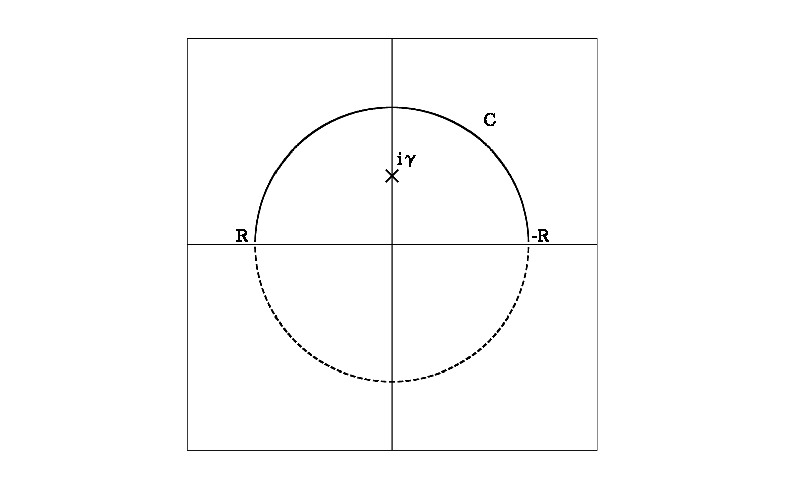
\includegraphics[width = 10cm]{./EPS/figure3new.eps}
  \label{fig3}
\end{figure}\\
極は$\omega = \pm i\gamma$で一位の極. 積分経路は上半円とする. 留数定理より
\begin{eqnarray}
  R(i\gamma) = \lim_{z\rightarrow i\gamma}(z - i\gamma)f(z) = \frac{C_Re^{\gamma t}}{2i\gamma}\label{R}
\end{eqnarray}
ここで$z = Re^{i\theta}$の変数変換を施すことにより
\begin{eqnarray}
  \int_{C_1}dz\frac{e^{-izt}}{(z^2 + \gamma^2)} = \int_0^\pi d\theta\frac{iRe^{-iRe^{i\theta}}t}{(R^2e^{2i\theta} + \gamma^2)}= \int_0^\pi d\theta\frac{iRe^{-iRt\cos\theta}e^{Rt\sin\theta}}{(R^2e^{2i\theta} + \gamma^2)}
\end{eqnarray}
かつ一般に$|\alpha + \beta| > |\alpha|-|\beta|$が成立することから
\begin{eqnarray}
  \left|\frac{iRe^{-iRt\cos\theta}e^{Rt\sin\theta}}{(R^2e^{2i\theta} + \gamma^2)}\right| < \frac{Re^{Rt\sin\theta}}{R^2 - \gamma^2}
\end{eqnarray}
これが$R\rightarrow\infty$で発散しないためには$t<0$である必要があるが, $t>0$の場合も発散しないようにしたい. そのためには$e^{-izt}\rightarrow e^{iz|t|}$とすればよい. つまり, (\ref{R})は
\begin{eqnarray}
  R(i\gamma) = \lim_{z\rightarrow i\gamma}(z - i\gamma)f(z) = \frac{C_Re^{-\gamma |t|}}{2i\gamma}\label{R2}
\end{eqnarray}
とするべきである. 以上からコーシーの積分定理より
\begin{eqnarray}
  C_v(t) = \frac{C_Re^{-\gamma|t|}}{2M^2\gamma}
\end{eqnarray}
となる. 同時刻($t = 0$)の相関は
\begin{eqnarray}
  C_v = \frac{C_R}{2M^2\gamma}
\end{eqnarray}
であり, 熱平衡状態のエネルギー等分配則
\begin{eqnarray}
  M\expval{v^2} = k_BT
\end{eqnarray}
を認めれば
\begin{eqnarray}
  C_R = 2k_BTM\gamma
\end{eqnarray}
となる. これはNyquistの定理と呼ばれ, 揺動散逸定理のひとつである.
\section{Born-Markov型量子マスター方程式}
熱浴と接している一次元調和振動子系のBorn-Markov型量子マスター方程式を解く.
\begin{itemize}
\item 系のハミルトニアンは調和振動子$H = \hbar\omega a^\dagger a$.
  
\item Born-Markov近似なので熱浴の密度演算子は時間発展せず, 回転波近似(弱結合)も有効.
  
\item マスター方程式は系の密度演算子の時間発展を与えている.\footnote{描像によっては生成消滅演算子も時間依存しそうである. 普通(?)マスター方程式を導出するときは相互作用描像を経由するので生成消滅演算子も一般に時間依存性を持つ. しかし今回は回転波近似が有効であるため, $a(t) = a(0)e^{-i\omega t}$のように分解できる. 後述のマスター方程式には$a^\dagger$, $a$がペアになって現れているので, マスター方程式には生成消滅演算子に依る時間依存性は現れない. $a^\dagger$, $a$がペアになっていないような項が現れたら生成消滅演算子由来の時間依存性を考慮しなければならないが, そもそもそういう項を落とすのがBorn-Markov近似である. }.
\end{itemize}
\begin{itemize}
\item 生成消滅演算子と粒子数状態
  
\item 交換関係の計算  
\end{itemize}
あたりの知識が必要です.
\subsection{問題設定}
量子マスター方程式が与えられている:
\begin{eqnarray}
  \nonumber  \partial_t\rho(t) = &-&i\omega[a^\dagger a, \rho(t)] + \kappa\overline{n}(2a^\dagger\rho(t)a - aa^\dagger\rho(t) - \rho(t)aa^\dagger)\\
  &+&\kappa(\overline{n} + 1)(2a\rho(t)a^\dagger - a^\dagger a\rho(t) - \rho(t)a^\dagger a)\label{master}
\end{eqnarray}
ただし
\begin{eqnarray}
  \kappa > 0,\hspace{1cm} \overline{n} = \frac{1}{e^{\hbar\omega/kT}-1},\hspace{1cm} [a, a^\dagger] = 1
\end{eqnarray}
であり, $\kappa$は減衰定数, $\overline{n}$はBose-Einstein分布関数, $a, a^\dagger$は生成消滅演算子である.
\subsection{熱平衡(問題1)}
熱浴の温度が$T$であることから, 系の温度を$T$とする有限温度系を考えればそれが熱平衡状態にあることは明らか. 平衡状態なので密度演算子が系のハミルトニアンを用いて
\begin{eqnarray}
  \rho_{th} = \frac{e^{-H/kT}}{{\rm Tr}e^{-H/kT}}\label{equiliblium}
\end{eqnarray}
と書ける. (\ref{equiliblium})の分母は規格化条件であり,以下のように計算できる\footnote{トレースは直行完全系ではさんで和を取ればいい.規格化は後でできるので, 正規直行完全系でなくてもいいらしい. つまりどんな完全系を選んできても規格化係数を除けば同じ結論に辿り着く. 今回は明らかに$a^\dagger a$の固有状態$\ket{n}$を用いるのが簡単. }(以下, 逆温度$1/kT$を$\beta$と置き換えています):
\begin{eqnarray}
  \nonumber  {\rm Tr}e^{-\beta\hbar\omega a^\dagger a} &=& \sum_{n}\bra{n}e^{-\beta\hbar\omega a^\dagger a}\ket{n}\\
  \nonumber  &=& \sum_{n}e^{-\beta\hbar\omega n}\\
  &=& \frac{1}{1-e^{-\beta\hbar\omega}} = (\overline{n} -1)
\end{eqnarray}

密度演算子はLiouville-von Neumann方程式を満たす:
\begin{eqnarray}
  i\hbar\partial_t\rho_{th} &=& [H, \rho_{th}]\\
  &=& \frac{\hbar\omega}{\overline{n}-1}[a^\dagger a, e^{\beta\hbar\omega a^\dagger a}]\label{commutation}
\end{eqnarray}
$[A, [B, A]] = [B, [B, A]] = 0$が成立しているときに$[B, e^{\lambda A}] = \lambda[B, A]e^{\lambda A}$であることを利用して\footnote{証明してみよう!}
\begin{eqnarray}
  (\ref{commutation}) = \frac{\hbar\omega}{\overline{n}-1}\beta\hbar\omega[a^\dagger a, a^\dagger a]e^{\beta\hbar\omega a^\dagger a} = 0
\end{eqnarray}
したがって, $\rho_{th}$の時間微分がゼロであることから時間発展しない熱平衡状態であることがわかる\footnote{式(\ref{master})を使っていないが良いのか?と思うかもしれないが, そもそも量子マスター方程式を導出するときはLiouville-von Neumann方程式からスタートするので, QME$\subset$LvNEである}.
\subsection{調和振動子のエネルギー(問題2)}
続いて式(\ref{master})を用いてエネルギー期待値の時間発展を追う.物理量の期待値はハミルトニアンに密度演算子を掛けてトレースアウトすればよい\footnote{本来, 密度演算子を用いた物理量の期待値は$\expval{A} = \frac{{\rm Tr}A\rho(t)}{{\rm Tr}\rho(t)}$で記述されるが, 今回は${\rm Tr}\rho(t) = 1$を課している.つまり$\rho(t)$が規格化されているという条件である.}:
\begin{eqnarray}
  \partial_tE(t) = \partial_t{\rm Tr}[H\rho(t)] = \hbar\omega\partial_t\sum_n \bra{n}a^\dagger a\rho(t)\ket{n} = \hbar\omega\partial_t\sum_nn\bra{n}\rho(t)\ket{n}\label{4.1}
\end{eqnarray}
また, 式(\ref{master})に左から$H = \hbar\omega a^\dagger a$を掛けてトレースアウトする:
\begin{eqnarray}
  \nonumber  \partial_tE(t) = &-&i\hbar\omega^2\underline{{\rm Tr}\left(a^\dagger a[a^\dagger a, \rho(t)]\right)}_{\rm 1} + \kappa\overline{n}\hbar\omega\left(2\underline{{\rm Tr}a^\dagger aa^\dagger\rho(t)a}_{\rm 2} - \underline{{\rm Tr}a^\dagger a aa^\dagger\rho(t)}_{\rm 3} - \underline{{\rm Tr}a^\dagger a\rho(t)aa^\dagger}_{\rm 4}\right)\\
  &+&\kappa(\overline{n} + 1)\hbar\omega\left(2\underline{{\rm Tr}a^\dagger aa\rho(t)a^\dagger}_5 - \underline{{\rm Tr}a^\dagger aa^\dagger a\rho(t)}_6 - \underline{{\rm Tr}a^\dagger a\rho(t)a^\dagger a}_7\right)\label{ModifiedMaster}
\end{eqnarray}
式(\ref{ModifiedMaster})の右辺は,
\begin{eqnarray}
  \nonumber  1.\hspace{5mm}{\rm Tr}\left(a^\dagger a[a^\dagger a, \rho(t)]\right) &=& {\rm Tr}\left[a^\dagger a(a^\dagger a\rho(t)-\rho(t)a^\dagger a)\right]\\
  \nonumber  &=&\sum_n\left[\bra{n}a^\dagger aa^\dagger a\rho(t)\ket{n} - \bra{n}a^\dagger a\rho(t)a^\dagger a\ket{n}\right]\\
  &=&\sum_n\left[n^2\bra{n}\rho(t)\ket{n} - n^2\bra{n}\rho(t)\ket{n}\right] = 0\\
  2.\hspace{5mm}{\rm Tr}a^\dagger aa^\dagger\rho(t)a &=& \sum_n(n+1)^2\bra{n}\rho(t)\ket{n}\\
  3.\hspace{5mm}{\rm Tr}a^\dagger aaa^\dagger\rho(t) &=& \sum_nn(n+1)\bra{n}\rho(t)\ket{n}\\
  4.\hspace{5mm}{\rm Tr}a^\dagger a\rho(t)aa^\dagger &=& \sum_nn(n+1)\bra{n}\rho(t)\ket{n}\\
  5.\hspace{5mm}{\rm Tr}a^\dagger aa\rho(t)a^\dagger &=& \sum_n(n-1)n\bra{n}\rho(t)\ket{n}\\
  6.\hspace{5mm}{\rm Tr}a^\dagger aa^\dagger a\rho(t) &=& \sum_nn^2\bra{n}\rho(t)\ket{n}\\
  7.\hspace{5mm}{\rm Tr}a^\dagger a\rho(t)a^\dagger a &=& \sum_nn^2\bra{n}\rho(t)\ket{n}
\end{eqnarray}
用いて整理することができる\footnote{nの和については$n=0$とか$n=\infty$の境界を雑に扱っているように見えるが, ちゃんとDirichlet境界条件を考慮してあげれば問題は起きない(と思う)}:
\begin{eqnarray}
  \nonumber \partial_tE(t) &=& \sum_n2\hbar\omega\left[\kappa\overline{n}((n+1)^2-n(n+1)) + \kappa(\overline{n}+1)((n-1)n - n^2)\right]\bra{n}\rho(t)\ket{n}\\
  &=&\sum_n2\hbar\omega\left[\kappa\overline{n}(n+1) - \kappa(\overline{n}+1)n\right]\bra{n}\rho(t)\ket{n}\\
  &=&\sum_n2\hbar\omega\kappa\left(\overline{n} - n\right)\bra{n}\rho(t)\ket{n}
\end{eqnarray}
式(\ref{4.1})と比較すると
\begin{eqnarray}
  \hbar\omega\sum_n\partial_tn\bra{n}\rho(t)\ket{n} &=& \sum_n2\hbar\omega\kappa\left(\overline{n} - n\right)\bra{n}\rho(t)\ket{n}\\
  \partial_tn\bra{n}\rho(t)\ket{n} &=& 2\kappa\left(\overline{n} - n\right) \bra{n}\rho(t)\ket{n}\\
  &\therefore& n\bra{n}\rho(t)\ket{n} = C_ne^{2\kappa\left(\frac{\overline{n}}{n} - 1\right)t}
\end{eqnarray}
よってエネルギー固有値は式(\ref{4.1})より
\begin{eqnarray}
  E(t) = \sum_n C_ne^{2\kappa\left(\frac{\overline{n}}{n} - 1\right)t}
\end{eqnarray}
となる\footnote{熱平衡状態では物理量に温度が関与していそうだが, (平衡状態ではない)非平衡の形式では系の温度が式に現れていないことを不思議に思うかもしれない. しかし, そもそも温度とは平衡状態でなければ定義できない.むしろ平衡状態によって定義される量である. 熱力学においては温度という概念が当たり前のように存在するが, そもそもは熱力学第零法則に則って熱平衡の下で定義される(熱力学は平衡状態に関する理論). つまり我々は平衡有限温度系では式(\ref{equiliblium})を用いて温度を定義することになる. この式だけでは定義のしようがないと思うかもしれないが, 場の量子論の形式においては理論を閉じるようにうまく繰り込み条件を選ぶことにより,自己無同着的に定義されることになる.}.
$C_n$は積分定数\footnote{Cがn依存性を持っていないと式(\ref{4.16})が発散してしまう.}. 初期状態$t = 0$のエネルギー平均が$E(0)$であることから
\begin{eqnarray}
  E(0) = \sum_nn\bra{n}\rho(0)\ket{n} = \sum_nC_n\label{4.16}
\end{eqnarray}
となる. 
\subsection{位置・運動量平均の時間発展(問題3)}
(問題2)と同様にマスター方程式のトレースアウトで期待値を見積もる.以下, 位置と運動量は$m=\hbar=\omega = 1$で無次元化している\footnote{マスター方程式は無次元化されていないのでアンバランスなあまり良いnotationではない. 本来ならマスター方程式, $\overline{n}$も合わせて無次元化すべき.}.

生成消滅演算子の言葉で位置は$q = \frac{1}{\sqrt{2}}(a^\dagger + a)$と表されることを用いて
\begin{eqnarray}
  \nonumber  \partial_tq(t) &=& \frac{1}{\sqrt{2}}\partial_t{\rm Tr}(a^\dagger + a)\rho(t)\\
  &=& \frac{1}{\sqrt{2}}\partial_t\sum_n\left[\sqrt{n}\bra{n-1}\rho(t)\ket{n} + \sqrt{n+1}\bra{n+1}\rho(t)\ket{n}\right]\label{Position}
\end{eqnarray}
マスター方程式の右辺をトレースアウト:
\begin{eqnarray}
  \nonumber  (\ref{master}) &\rightarrow& \frac{1}{\sqrt{2}}\Bigl[-i\omega\underline{{\rm Tr}(a^\dagger +a)(a^\dagger a\rho(t) - \rho(t)a^\dagger a)}_1\\
    \nonumber    &+& \kappa\overline{n}\left(2\underline{{\rm Tr}(a^\dagger +a)a^\dagger \rho(t)a}_2 - \underline{{\rm Tr}(a^\dagger + a)aa^\dagger \rho(t)}_3 - \underline{{\rm Tr}(a^\dagger +a)\rho(t)aa^\dagger}_4\right)\\
    &+& \kappa(\overline{n}+1)\left(2\underline{{\rm Tr}(a^\dagger +a)a\rho(t)a^\dagger}_5 - \underline{{\rm Tr}(a^\dagger + a)a^\dagger a\rho(t)}_6 - \underline{{\rm Tr}(a^\dagger +a)\rho(t)a^\dagger a}_7\right)\Bigr]\label{position}
\end{eqnarray}
各項について整理:
\begin{eqnarray}
  &1.&\hspace{5mm}\sum_n\left[-\sqrt{n}\bra{n-1}\rho(t)\ket{n}+\sqrt{n+1}\bra{n+1}\rho(t)\ket{n}\right]\\
  &2.&\hspace{5mm}\sum_n\left[(n+1)\sqrt{n}\bra{n-1}\rho(t)\ket{n}+\sqrt{n+1}(n+2)\bra{n+1}\rho(t)\ket{n}\right]\\
  &3.&\hspace{5mm}\sum_n\left[n\sqrt{n}\bra{n-1}\rho(t)\ket{n}+\sqrt{n+1}(n+2)\bra{n+1}\rho(t)\ket{n}\right]\\
  &4.&\hspace{5mm}\sum_n\left[(n+1)\sqrt{n}\bra{n-1}\rho(t)\ket{n}+\sqrt{n+1}(n+1)\bra{n+1}\rho(t)\ket{n}\right]\\
  &5.&\hspace{5mm}\sum_n\left[(n-1)\sqrt{n}\bra{n-1}\rho(t)\ket{n}+n\sqrt{n+1}\bra{n+1}\rho(t)\ket{n}\right]\\
  &6.&\hspace{5mm}\sum_n\left[(n-1)\sqrt{n}\bra{n-1}\rho(t)\ket{n}+(n+1)\sqrt{n+1}\bra{n+1}\rho(t)\ket{n}\right]\\
  &7.&\hspace{5mm}\sum_n\left[n\sqrt{n}\bra{n-1}\rho(t)\ket{n}+n\sqrt{n+1}\bra{n+1}\rho(t)\ket{n}\right]
\end{eqnarray}
式(\ref{position})をまとめる:
\begin{eqnarray}
  \nonumber (\ref{position}) &=& \frac{1}{\sqrt{2}}\sum_n\Bigl[-i\omega\left(-\sqrt{n}\bra{n-1}\rho(t)\ket{n}+\sqrt{n+1}\bra{n+1}\rho(t)\ket{n}\right)\\
    \nonumber    &&+ \kappa\overline{n}\left( \sqrt{n}\bra{n-1}\rho(t)\ket{n}+\sqrt{n+1}\bra{n+1}\rho(t)\ket{n}\right)\\
    &&+ \kappa(\overline{n}+1)\left(-\sqrt{n}\bra{n-1}\rho(t)\ket{n}-\sqrt{n+1}\bra{n+1}\rho(t)\ket{n}\right)\Bigr]\label{positon2}\\
  &=& \frac{1}{\sqrt{2}}\sum_n\Bigl[\sqrt{n}\left(i\omega - \kappa\right)\bra{n-1}\rho(t)\ket{n}-\sqrt{n+1}\left(i\omega+\kappa\right)\bra{n+1}\rho(t)\ket{n} \Bigr]
\end{eqnarray}
(\ref{Position})と比較:
\begin{eqnarray}
  \sum_n \partial_t\bra{n-1}\rho(t)\ket{n} = \sum_n (i\omega - \kappa)\bra{n-1}\rho(t)\ket{n}\\
  \sum_n \partial_t\bra{n+1}\rho(t)\ket{n} = -\sum_n (i\omega + \kappa)\bra{n+1}\rho(t)\ket{n}
\end{eqnarray}
これを解くと
\begin{eqnarray}
  \bra{n-1}\rho(t)\ket{n} &=& C_1e^{(i\omega - \kappa)t}\\
  \bra{n+1}\rho(t)\ket{n} &=& C_2e^{-(i\omega + \kappa)t}
\end{eqnarray}
以上より
\begin{eqnarray}
  q &=& \frac{1}{\sqrt{2}}\sum_n\left[\sqrt{n}C_1e^{(i\omega - \kappa)t} + \sqrt{n+1}C_2e^{-(i\omega + \kappa)t}\right]\\
  \dot{q} &=& p = \frac{1}{\sqrt{2}}\sum_n\Bigl[\sqrt{n}C_1(i\omega - \kappa)e^{(i\omega - \kappa)t}- \sqrt{n+1}C_2(i\omega + \kappa)e^{-(i\omega + \kappa)t}\Bigr]\\
  \ddot{q} &=& \dot{p} = \frac{1}{\sqrt{2}}\sum_n\Bigl[\sqrt{n}C_1(i\omega - \kappa)^2e^{(i\omega - \kappa)t}- \sqrt{n+1}C_2(i\omega + \kappa)^2e^{-(i\omega + \kappa)t}\Bigr]
\end{eqnarray}
ここでは$\dot{q} = p$であることを用いている.以上から$\dot{p}, p, q$による微分方程式を立てる\footnote{ちょっと式とにらめっこしてれば簡単}:
\begin{eqnarray}
  \dot{p} = -(\omega^2 + \kappa^2)q -2\kappa p
\end{eqnarray}

右辺第2項が速度に比例する減衰を表している.角振動数に$\kappa$が入っており, 減衰の幅が増加するほど角振動数も大きくなる. 古典的な減衰振動を摩擦のあるばねの振動と解釈する場合, 角振動数は減衰(摩擦)がない場合と変わらないはずなので, 古典と完全には対応していないように見える.
一方で, 減衰をエネルギーの散逸と捉えるならば, 低温の熱浴からの影響で角振動数が大きくなるという解釈は, 低温ではばね定数が大きくなる古典的な解釈と一致する.

きれいになったとはいえまだミスがないか不安です...
\subsection{数値計算}
問題2の和が計算しきれなかったので, 数値計算で(\ref{4.16})が本当に緩和するかどうかを確認.
\begin{figure}[htbp]
  \begin{minipage}{0.5\hsize}
    \centering
    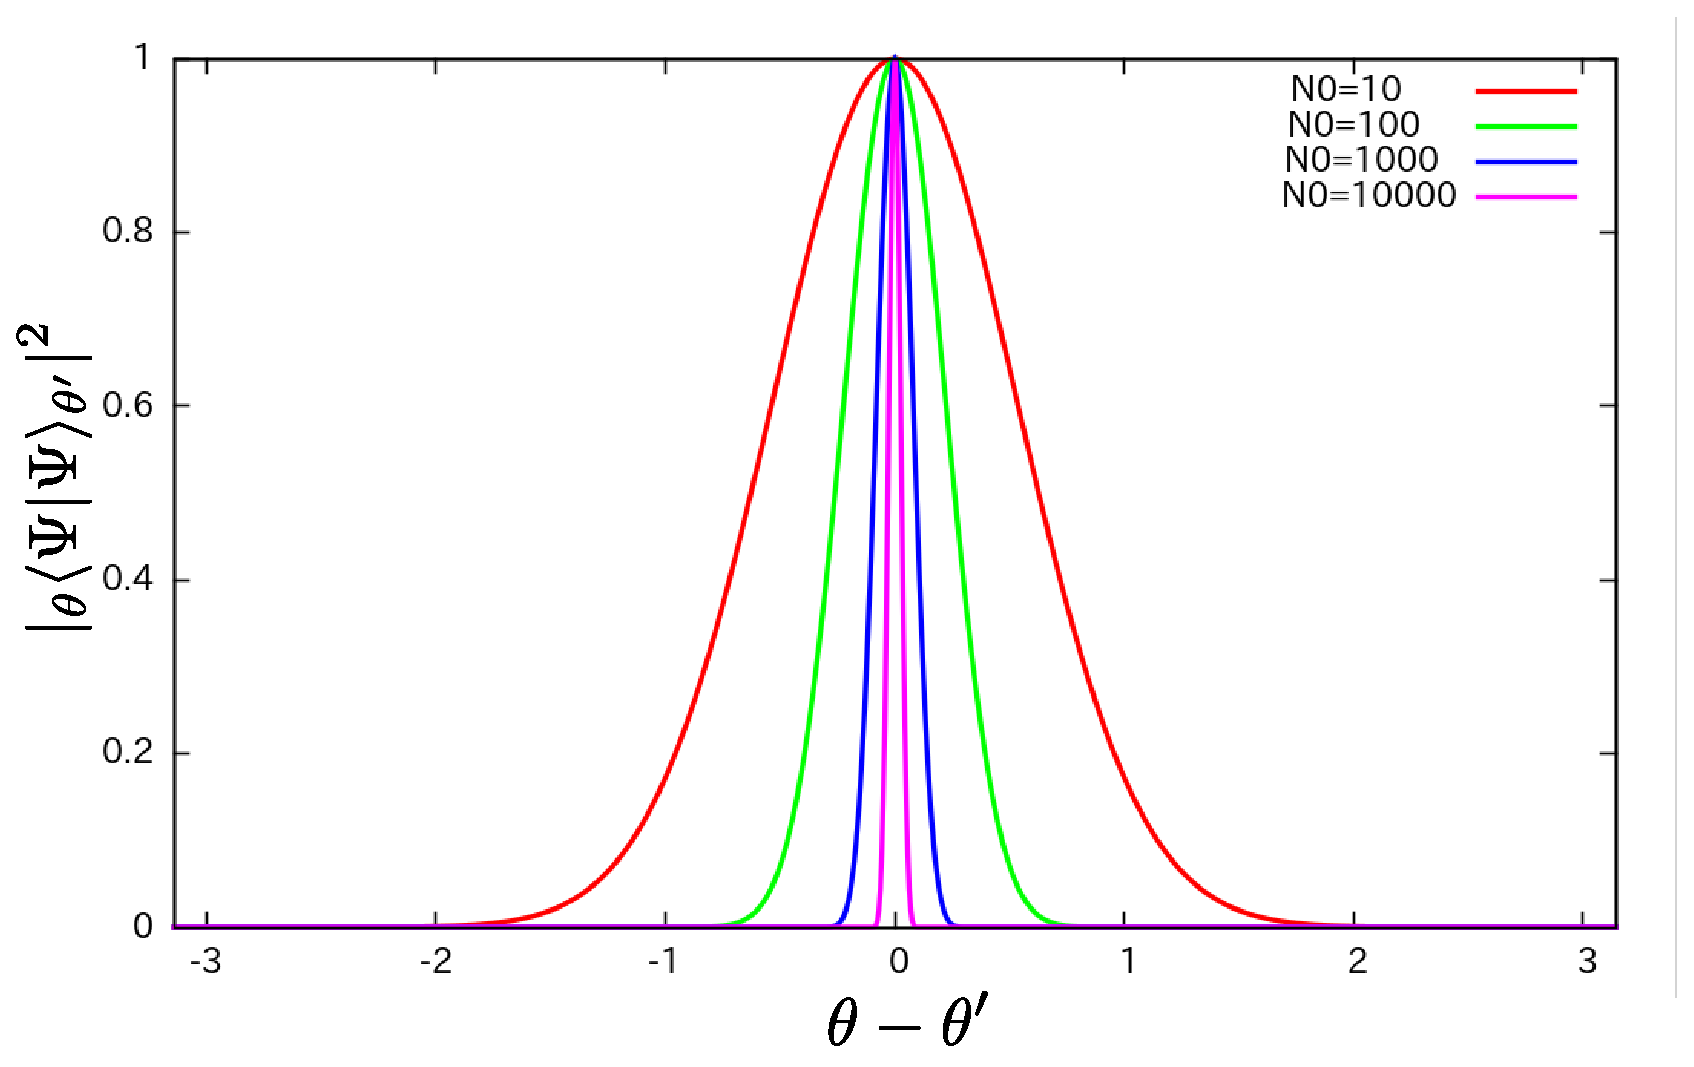
\includegraphics[width = 7cm]{./EPS/fig1.eps}
    \figcaption{$\kappa = \overline{n} = 1$}
    \label{fig1}
  \end{minipage}
  \begin{minipage}{0.5\hsize}
    \centering
    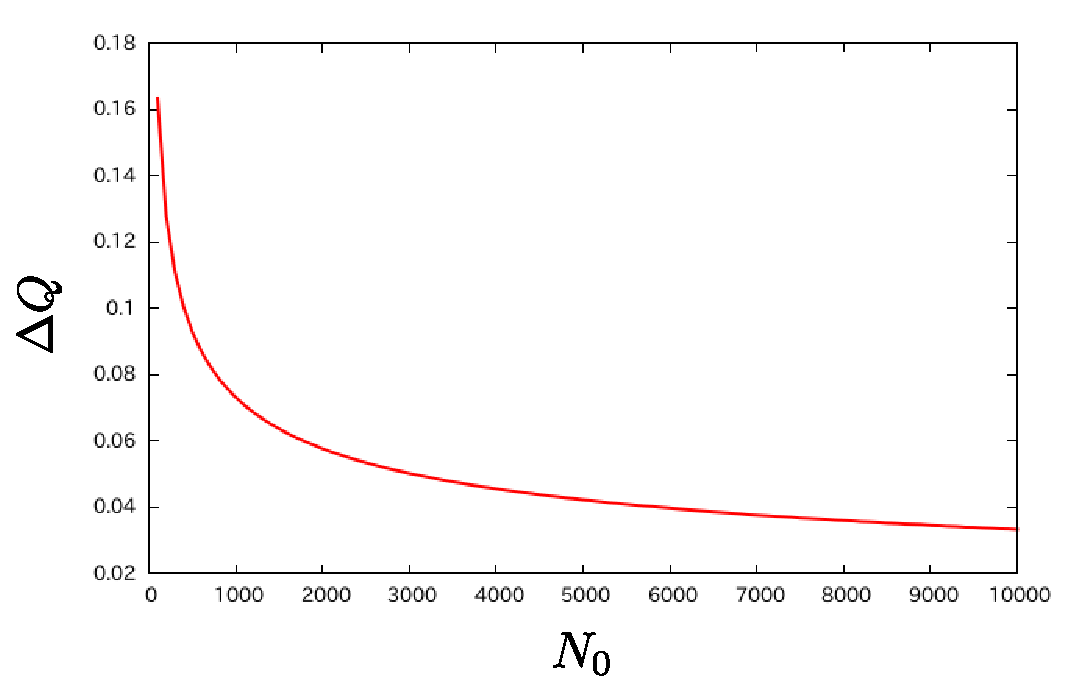
\includegraphics[width = 7cm]{./EPS/fig2.eps}
    \figcaption{$\kappa$が負の場合}
    \label{fig2}
  \end{minipage}
\end{figure}
$E(0)$の情報は$C_n$に組み込まれており, さらに$C_n$の関数列の形に制限は収束すること以外には特にない. $E(0)$は$C_n$の汎関数だとも言える. つまり, $C_n$の与え方によって熱浴を通じてエネルギーが流出するか流入するかが決まる\footnote{系の初期温度が熱浴の温度$T$より大きければ流出するし,逆なら流入するのが普通. 非平衡状態では温度は定義できないので, 正確には流入・流出を支配しているのは温度ではなくエントロピーである.}. 汎関数は無限個の自由度を持つ関数なので$E(0)$は単なる系のエネルギーの初期値だけでなく,熱浴との相関具合などの自由度を含んでいる(かもしれない). 図1にエネルギーが緩和する様子を示した.今回は$C_n = \frac{1}{n^2}, -\frac{1}{n^2} + \frac{5}{2n^5}$の2つを計算. これは単に流入と流出を見たかったために選んできたものであり, $C_n$が収束するような関数列を選べば緩和は観測できるはず.

また, $\kappa$が負の場合, 振幅は減衰することなく増幅することを図2で確認している.
\section{線形応答理論}
\subsection{概要}
ある平衡系に$t = t_0$で何かしらの外場がかかったときの非平衡過程を見る理論. 摂動1次までの応答を見るので線形応答と呼ばれる.
\subsection{線形応答理論の基本概念}
平衡系のハミルトニアンを$H$, 外場$H_{\rm ex}(t)$としてFull Hamiltonian
\begin{eqnarray}
 H_{T} = H + H_{\rm ex}(t)
\end{eqnarray}
を考える. $H_{\rm ex}(t)$は$t< t_0$においてはゼロである. 平衡系の時間依存Schr\"odinger方程式:
\begin{eqnarray}
  i\partial_t\ket{\psi(t)} = H\ket{\psi(t)}
\end{eqnarray}
に対して外場を加えたSchr\"odinger方程式:
\begin{eqnarray}
  i\partial_t\ket{\Psi(t)} = \qty(H + H_{\rm ex}(t))\ket{\Psi(t)}
\end{eqnarray}
がある. $\ket{\Psi(t)}$は非平衡系の状態である. 平衡系の形式解が
\begin{eqnarray}
  \ket{\psi(t)} = e^{-iHt}\ket{\psi(0)}
\end{eqnarray}
であることから, ユニタリー演算子を用いて$\ket{\Psi(t)}$が
\begin{eqnarray}
  \ket{\Psi(t)} = e^{-iHt}U(t)\ket{\psi(0)}
\end{eqnarray}
と書けるものとする. これをSchr\"odinger方程式に代入すると
\begin{eqnarray}
  i\partial_t U(t) = e^{iHt}H_{\rm ex}(t)e^{-iHt}U(t) = H'_{\rm ex}(t)U(t)
\end{eqnarray}
という$U(t)$の時間発展方程式が得られる. ここで$H'_{\rm ex}(t)$は$H$による$H_{\rm ex}(t)$のHeisenberg描像になっている. 相互作用描像のときの議論と同様に
\begin{eqnarray}
  U(t) = 1 (t < t_0)
\end{eqnarray}
という条件を課すと
\begin{eqnarray}
  U(t) = 1 -i\int_{t_0}^{t}dt_1H'_{\rm ex}(t_1) + (-i)^2\int_{t_0}^{t}dt_1\int_{t_0}^{t_1}dt_2H'_{\rm ex}(t_1)H'_{\rm ex}(t_2) + \cdots
\end{eqnarray}
が得られる. 外場に対して1次のオーダーのみを扱うことにすると, 状態は
\begin{eqnarray}
  \ket{\Psi(t)} = e^{-iHt}\ket{\psi(0)} -ie^{-iHt}\int_{t_0}^{t}dt_1H'_{\rm ex}(t_1)\ket{\psi(0)}
\end{eqnarray}
となる. これを用いて任意の演算子$O(t)$(Schr\"odinger描像)の期待値は
\begin{eqnarray}
  \bra{\Psi(t)}O(t)\ket{\Psi(t)} &=& \bra{\psi(0)}\qty(1 + i\int_{t_0}^{t}dt_1H'_{\rm ex}(t_1))e^{iHt}O(t)e^{-iHt}\qty(1 - i\int_{t_0}^{t}dt_1H'_{\rm ex}(t_1))\ket{\psi(0)}\\
  &=& \bra{\psi(0)}O'(t)\ket{\psi(0)} + i\bra{\psi(0)}\int_{t_0}^{t}dt_1\qty[H'_{\rm ex}(t_1), O'(t)]\ket{\psi(0)} + \cdots
\end{eqnarray}
$O'(t) = e^{iHt}O(t)e^{-iHt}$であり, これまた$H$によるHeisenberg描像である. 外場が無い場合の期待値との差は$\ket{\psi_S(t)} = e^{-iH(t-t_0)}\ket{\psi_H(t_0)}$を用いて
\begin{eqnarray}
\nonumber  \delta\bra{\Psi(t)}O(t)\ket{\Psi(t)} &=& \bra{\Psi(t)}O(t)\ket{\Psi(t)} - \bra{\psi(t)}O(t)\ket{\psi(t)}\\
\nonumber  &=& \bra{\Psi(t)}O(t)\ket{\Psi(t)} - \bra{\psi(0)}e^{iHt}O(t)e^{-iHt}\ket{\psi(0)}\\
\nonumber  &=& \bra{\Psi(t)}O(t)\ket{\Psi(t)} - \bra{\psi(0)}O'(t)\ket{\psi(0)}\\
  &=& i\bra{\psi(0)}\int_{t_0}^{t}dt_1\qty[H'_{\rm ex}(t_1), O'(t)]\ket{\psi(0)}\label{linear-zero}
\end{eqnarray}
外場が弱いと仮定して一次のオーダーまでその寄与を見ようというのが線形応答理論(linear response theory, 久保理論). 上式は描像がごちゃまぜになっているように見えるがSchr\"odinger描像とHeisenberg描像は
\begin{eqnarray}
  \ket{\psi(0)}_S = \ket{\psi(0)}_H
\end{eqnarray}
という関係にあるのであえてラベル付けをしていない.
\subsection{有限温度系へ}
次に(\ref{linear-zero})を有限温度の期待値に拡張する. これは単純に期待値の取り方を変えれば良い:
\begin{eqnarray}
  \delta\ev{O(t)} = \frac{\sum_j e^{\beta H_j}\delta\ev{O(t)}{i}}{\sum_j e^{\beta H_j}} = \frac{\Tr[\rho \delta O(t)]}{\Tr[\rho]} = i\int_{t_0}^{t}dt_1 \Tr\qty(\rho [H'_{\rm ex}(t_1), O'(t)])
\end{eqnarray}
ここで重要なことは(\ref{linear-zero})を見てもわかる通り, 非平衡系を記述するのに平衡系の情報しか用いていないことである. 逆を言えば取り扱いの難しい非平衡系の相互作用みたいな項は2次のオーダーから効いてくるということである\footnote{平衡系から大きくずれた非平衡系を取り扱うのに線形応答理論は不適切である. 尤も, そのような非平衡系の取り扱いはまだ明確に確立されていない. 量子マスター方程式は線形応答を超える枠組みとして期待されている.}. 線形応答は非平衡系のとても簡単な取り扱いの方法になっている.
\subsection{簡単な例}
$t = t_0$での外場の影響を
\begin{eqnarray}
  H_{\rm ex}(t) = \int d\bm{x} J(\bm{x}, t)\phi(\bm{x}, t)
\end{eqnarray}
のような形で考える. $J$はただのc-数で$\phi$は実スカラー場. 場の演算子$\phi(\bm{x}, t)$の熱平均を見ると
\begin{eqnarray}
  \delta\ev{\phi(\bm{x}, t)} &=& i\int_{t_0}^{t}dt_1 \Tr\qty(\rho\int d\bm{x}_1 \qty[J(\bm{x}_1, t_1)\phi'(\bm{x}_1, t_1), \phi'(\bm{x}, t)])\\
  &=& -i\int_{t_0}^{t}dt_1\int d\bm{x}_1J(\bm{x}_1, t_1)\Tr\qty(\rho\qty[\phi(\bm{x}, t), \phi'(\bm{x}_1, t_1)])\label{linear-temp}
\end{eqnarray}
ここでトレース部分はグリーン関数(2点相関関数)の定義になっている. 密度行列が規格化されていると仮定すると温度グリーン関数は
\begin{eqnarray}
  iD(\bm{x}, t; \bm{x}_1, t_1) =\ev{T\qty[\phi'(\bm{x}, t)\phi'(\bm{x}_1, t_1)]} = \Tr\qty[\rho T\qty(\phi(\bm{x}, t)\phi(\bm{x}_1, t_1))]
\end{eqnarray}
であり, 遅延グリーン関数を
\begin{eqnarray}
  iD_R(\bm{x}, t; \bm{x}_1, t_1) = \ev{[\phi'(\bm{x}, t), \phi'(\bm{x}_1, t_1)]}\theta(t-t_1) = \Tr\qty(\rho[\phi'(\bm{x}, t), \phi'(\bm{x}_1, t_1)])\theta(t-t_1)
\end{eqnarray}
と定義すれば(\ref{linear-temp})はこれを用いて
\begin{eqnarray}
  \delta\ev{\phi(\bm{x}, t)} &=& -\int_{-\infty}^\infty dt_1\int d\bm{x} D_R(\bm{x}, t; \bm{x}_1, t_1)J(\bm{x}_1, t_1)\\
  &=& -\int d^4xD_R(\bm{x}, t; \bm{x}_1, t_1)J(\bm{x}_1, t_1)
\end{eqnarray}
とまとめることができる. 時間$t$をまとめて4元ベクトルにしてしまっているが, 遅延グリーン関数の$\theta$関数で$t$が負のところは消えるので問題はない.

さて, これを今度は運動量表示に持っていく. 外場を加えているものの時間は平衡系のハミルトニアン$H$で発展しているので, 空間の一様性は保たれていると考える\footnote{もちろんこれは線形部分までしか考えていないから. }. $D_R, J$それぞれをフーリエ変換すると
\begin{eqnarray}
  D_R(\bm{x}, t; \bm{x}_1, t_1) &=& \int\frac{d^4p}{(2\pi)^4} e^{-ip(x-x_1)}D_R(\bm{p}, p_0)\\
  J(\bm{x}_1, t_1) &=& \int\frac{d^4p'}{(2\pi)^4}e^{-ip'x_1}J(\bm{p}', p'_0)
\end{eqnarray}
これを代入すると
\begin{eqnarray}
  \delta\ev{\phi(\bm{x}, t)} &=& -\int \frac{d^4p}{(2\pi)^4} e^{-ipx}J(\bm{p}, p_0)D_R(\bm{p}, p_0)\\
  \delta\ev{\phi(\bm{p}, p_0)} &=& -J(\bm{p}, p_0)D_R(\bm{p}, p_0)
\end{eqnarray}
というとても簡単な形に落ち着く. 結論としては, 外場の影響による熱平均の変化は運動量空間において外場のSource$J$と遅延グリーン関数$D_R$\footnote{これも当然, 外場のないときの遅延グリーン関数である. }を掛けたものになる.

